\chapter{Similariteit}

Een similariteitsmaat voor afbeeldingen is in staat om de gelijkenis tussen twee gegeven
afbeelding uit te drukken als een getal uit het interval $[0,1]$. Dit getal nadert naar 1
naarmate de gelijkenis groter is. Bijgevolg kunnen we een dergelijke maat gebruiken om
een lijst van zoekresultaten te herordenen volgens similariteit met een bepaalde 
voorbeeld-afbeelding uit die lijst. In dit onderdeel van deze scriptie gaan we op zoek naar 
similariteitsmaten die geschikt zijn voor deze taak.

\section{Evaluatie van performantie}

Om uit meerdere similariteitsmaten de meest geschikte te kiezen, 
moeten we een manier vinden om een dergelijke maat objectief te beoordelen. 
Dit zullen we doen door elke
maat, voor een bepaalde voorbeeld-afbeelding, toe te passen op een eenzelfde collectie 
van afbeeldingen. Vervolgens zullen we de rangschikking die we zo bekomen
beoordelen met behulp van een performantiemaat.



\begin{figure}[p]
\begin{center}
%\subfigure[]{
%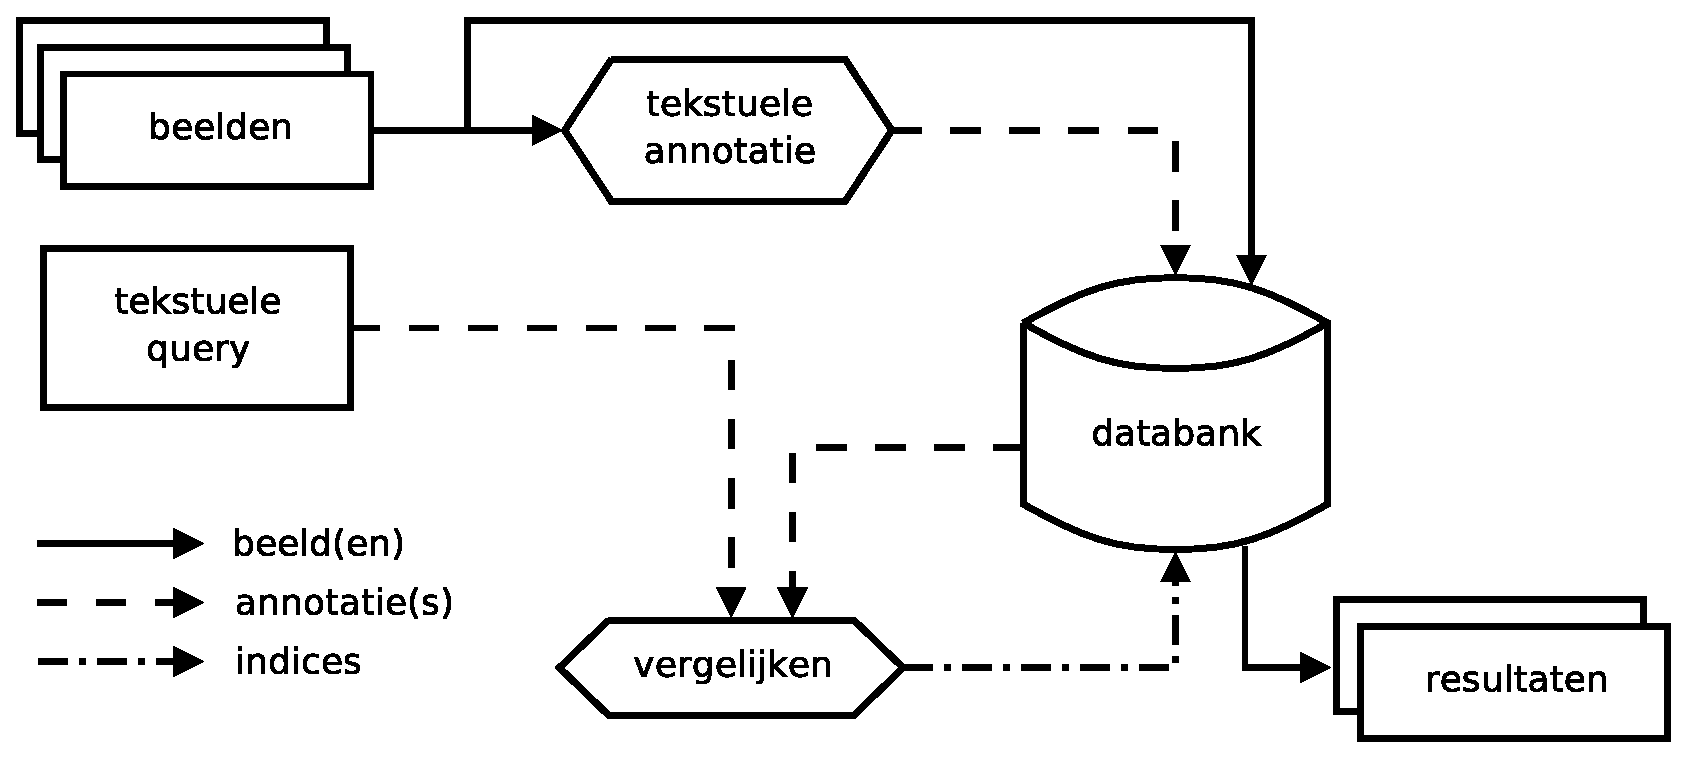
\includegraphics[width=10cm]{images/tbir.eps}
%\label{fig:tbir}
%}
%\subfigure[]{
%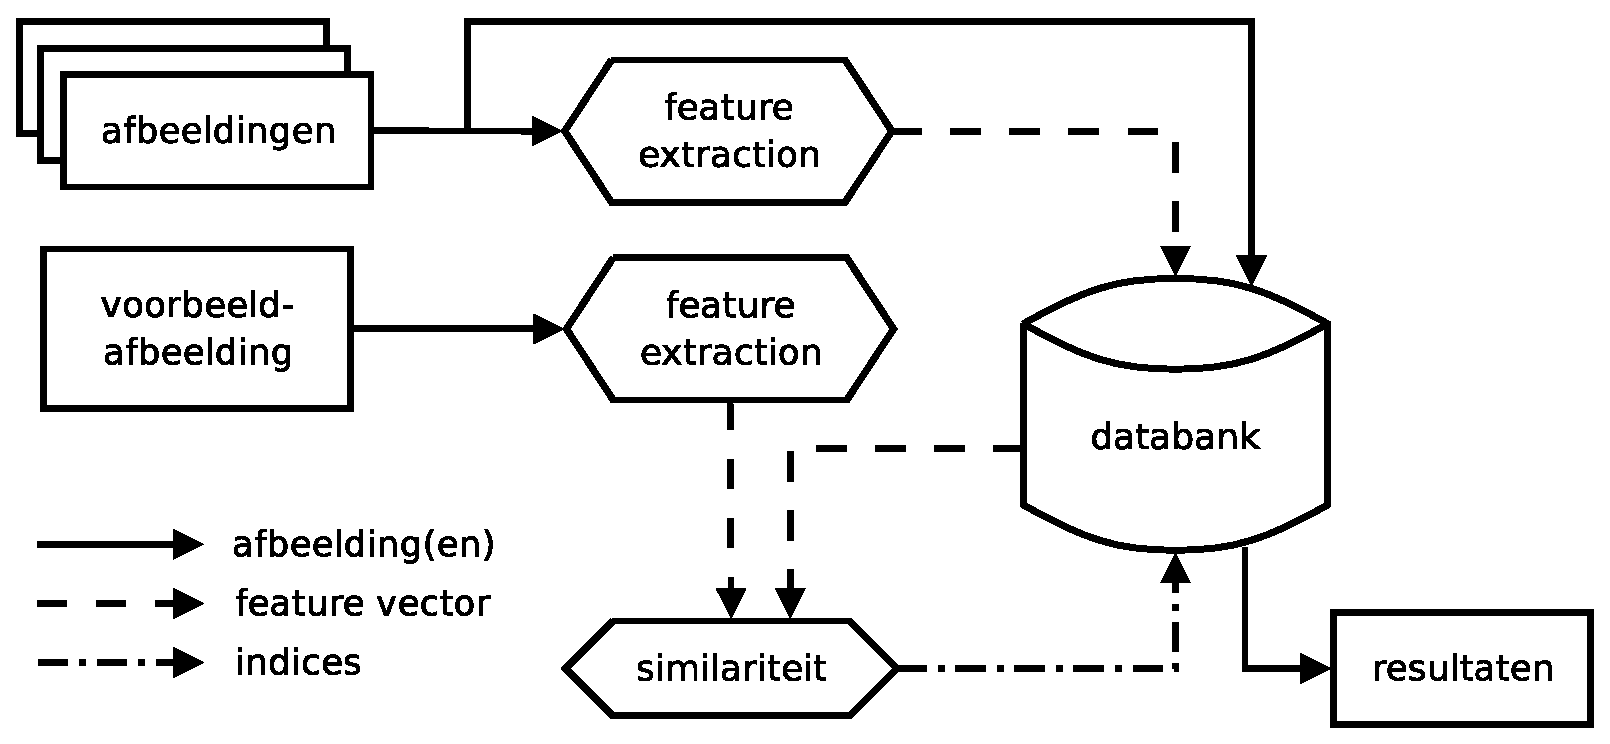
\includegraphics[width=10cm]{images/cbir.eps}
%\label{fig:cbir}
%}
\begin{tabular}{cccccc}

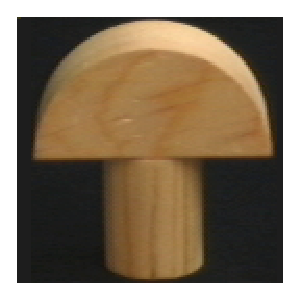
\includegraphics[width=2cm]{coil/beeld-0.eps} &
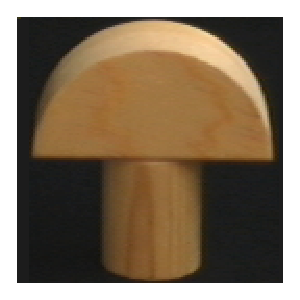
\includegraphics[width=2cm]{coil/beeld-1.eps} &

\includegraphics[width=2cm]{coil/beeld-2.eps} &
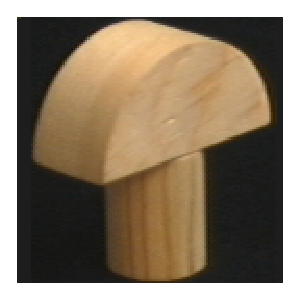
\includegraphics[width=2cm]{coil/beeld-3.eps} &
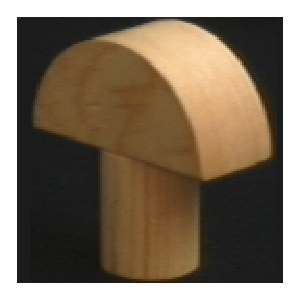
\includegraphics[width=2cm]{coil/beeld-4.eps} &
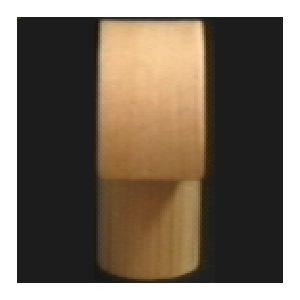
\includegraphics[width=2cm]{coil/beeld-5.eps} \\

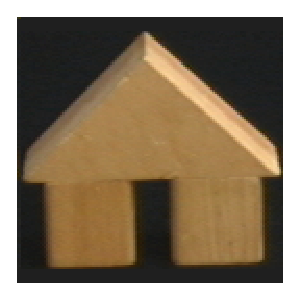
\includegraphics[width=2cm]{coil/beeld-42.eps} &
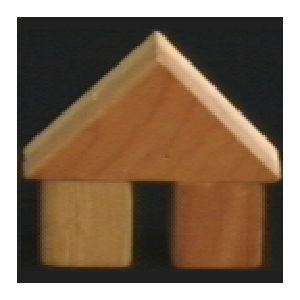
\includegraphics[width=2cm]{coil/beeld-43.eps} &
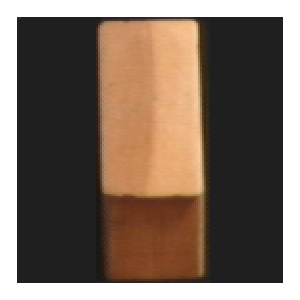
\includegraphics[width=2cm]{coil/beeld-44.eps} &
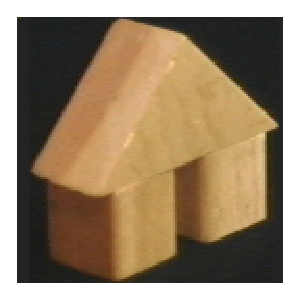
\includegraphics[width=2cm]{coil/beeld-45.eps} &
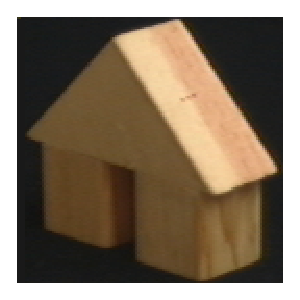
\includegraphics[width=2cm]{coil/beeld-46.eps} &
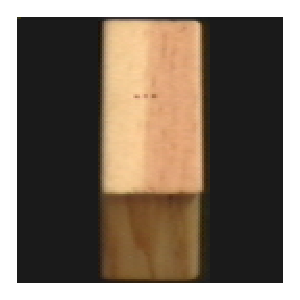
\includegraphics[width=2cm]{coil/beeld-47.eps} \\

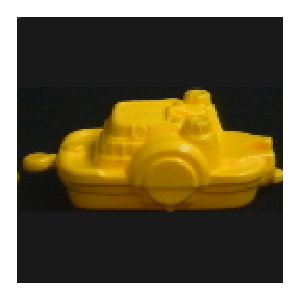
\includegraphics[width=2cm]{coil/beeld-12.eps} &
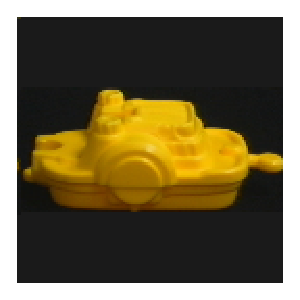
\includegraphics[width=2cm]{coil/beeld-13.eps} &
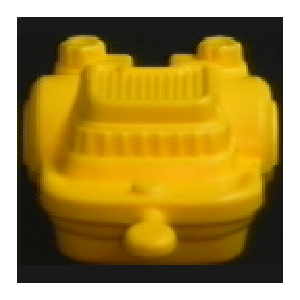
\includegraphics[width=2cm]{coil/beeld-14.eps} &
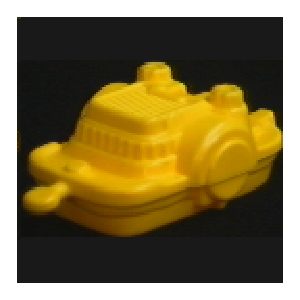
\includegraphics[width=2cm]{coil/beeld-15.eps} &
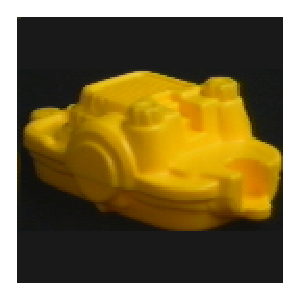
\includegraphics[width=2cm]{coil/beeld-16.eps} &
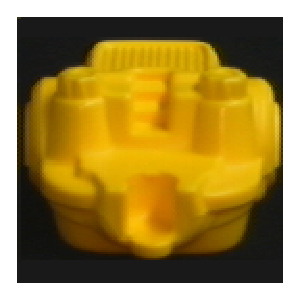
\includegraphics[width=2cm]{coil/beeld-17.eps} \\


\includegraphics[width=2cm]{coil/beeld-18.eps} &

\includegraphics[width=2cm]{coil/beeld-19.eps} &
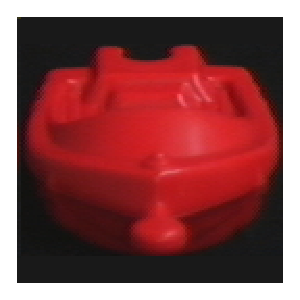
\includegraphics[width=2cm]{coil/beeld-20.eps} &
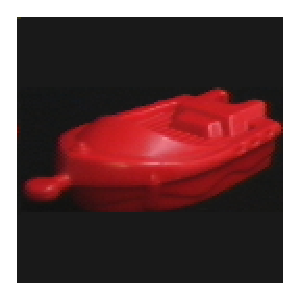
\includegraphics[width=2cm]{coil/beeld-21.eps} &
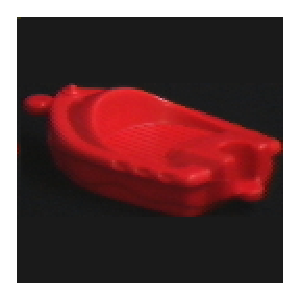
\includegraphics[width=2cm]{coil/beeld-22.eps} &
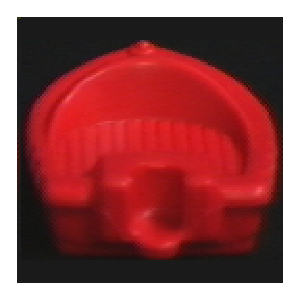
\includegraphics[width=2cm]{coil/beeld-23.eps} \\

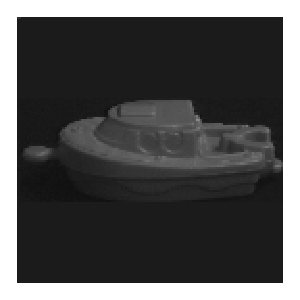
\includegraphics[width=2cm]{coil/beeld-24.eps} &
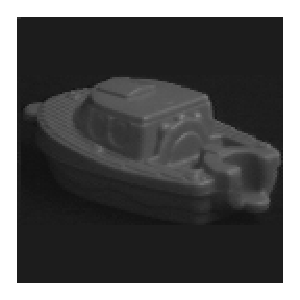
\includegraphics[width=2cm]{coil/beeld-25.eps} &
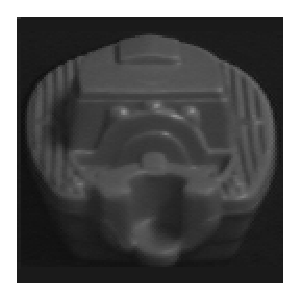
\includegraphics[width=2cm]{coil/beeld-26.eps} &
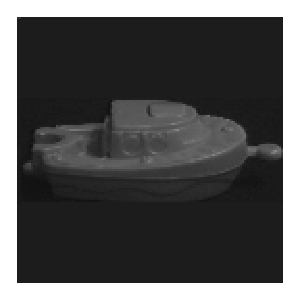
\includegraphics[width=2cm]{coil/beeld-27.eps} &
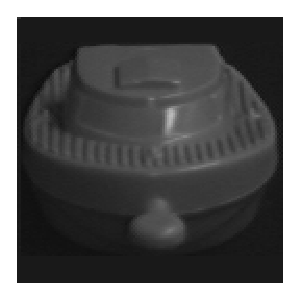
\includegraphics[width=2cm]{coil/beeld-28.eps} &
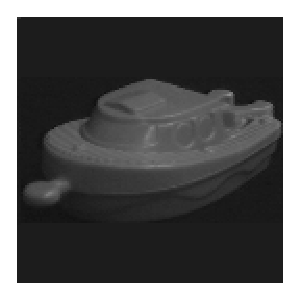
\includegraphics[width=2cm]{coil/beeld-29.eps} \\

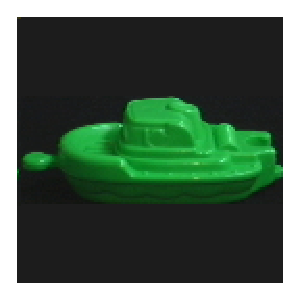
\includegraphics[width=2cm]{coil/beeld-54.eps} &
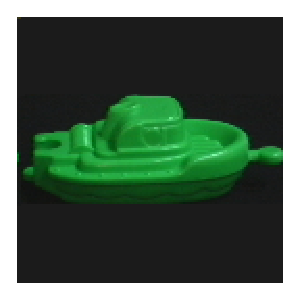
\includegraphics[width=2cm]{coil/beeld-55.eps} &
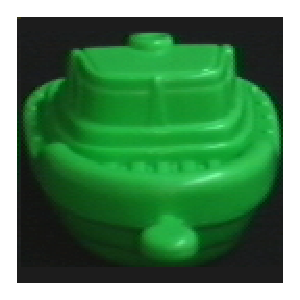
\includegraphics[width=2cm]{coil/beeld-56.eps} &
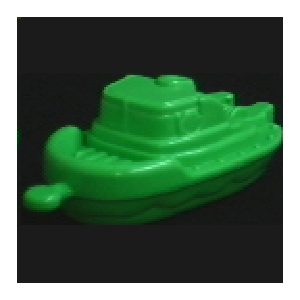
\includegraphics[width=2cm]{coil/beeld-57.eps} &
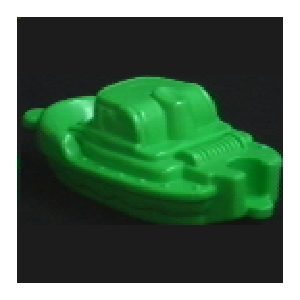
\includegraphics[width=2cm]{coil/beeld-58.eps} &
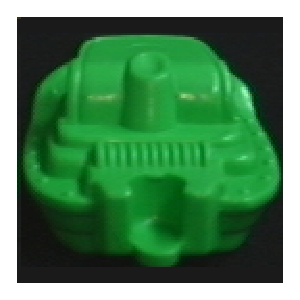
\includegraphics[width=2cm]{coil/beeld-59.eps} \\

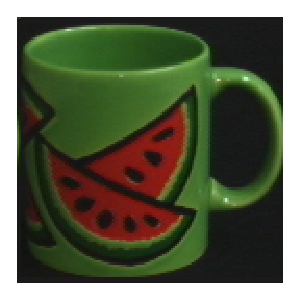
\includegraphics[width=2cm]{coil/beeld-30.eps} &
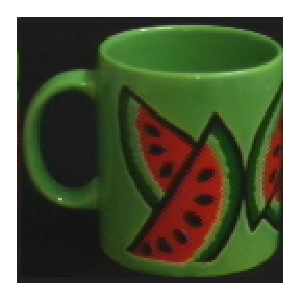
\includegraphics[width=2cm]{coil/beeld-31.eps} &
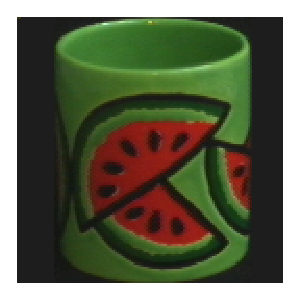
\includegraphics[width=2cm]{coil/beeld-32.eps} &
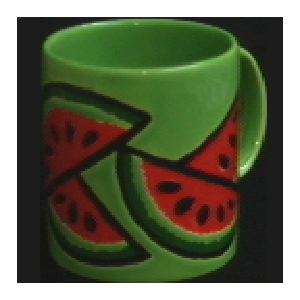
\includegraphics[width=2cm]{coil/beeld-33.eps} &
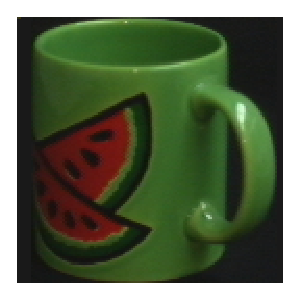
\includegraphics[width=2cm]{coil/beeld-34.eps} &
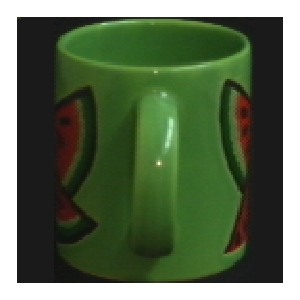
\includegraphics[width=2cm]{coil/beeld-35.eps} \\

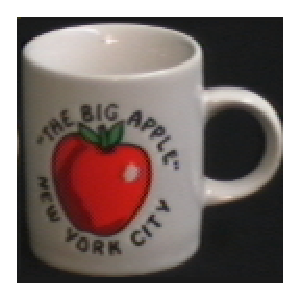
\includegraphics[width=2cm]{coil/beeld-36.eps} &
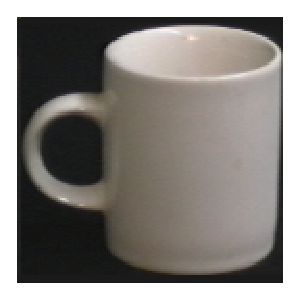
\includegraphics[width=2cm]{coil/beeld-37.eps} &
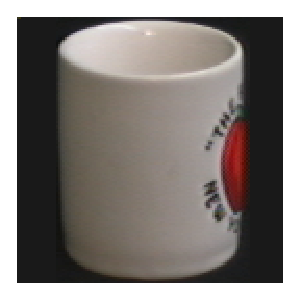
\includegraphics[width=2cm]{coil/beeld-38.eps} &
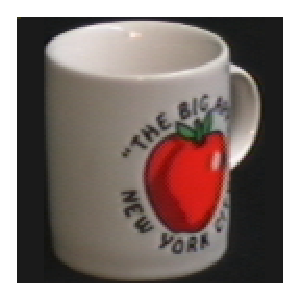
\includegraphics[width=2cm]{coil/beeld-39.eps} &
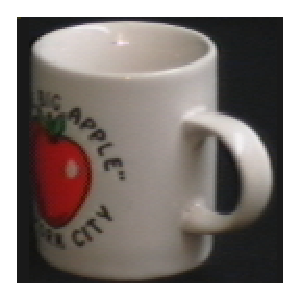
\includegraphics[width=2cm]{coil/beeld-40.eps} &
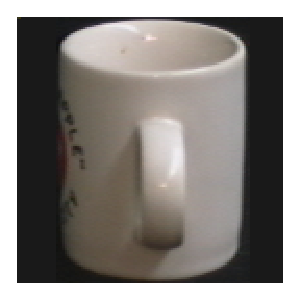
\includegraphics[width=2cm]{coil/beeld-41.eps} \\

\includegraphics[width=2cm]{coil/beeld-6.eps} &
\includegraphics[width=2cm]{coil/beeld-7.eps} &
\includegraphics[width=2cm]{coil/beeld-8.eps} &
\includegraphics[width=2cm]{coil/beeld-9.eps} &
\includegraphics[width=2cm]{coil/beeld-10.eps} &
\includegraphics[width=2cm]{coil/beeld-11.eps} \\

\includegraphics[width=2cm]{coil/beeld-48.eps} &
\includegraphics[width=2cm]{coil/beeld-49.eps} &
\includegraphics[width=2cm]{coil/beeld-50.eps} &
\includegraphics[width=2cm]{coil/beeld-51.eps} &
\includegraphics[width=2cm]{coil/beeld-52.eps} &
\includegraphics[width=2cm]{coil/beeld-53.eps} \\

\includegraphics[width=2cm]{coil/beeld-60.eps} &
\includegraphics[width=2cm]{coil/beeld-61.eps} &
\includegraphics[width=2cm]{coil/beeld-62.eps} &
\includegraphics[width=2cm]{coil/beeld-63.eps} &
\includegraphics[width=2cm]{coil/beeld-64.eps} &
\includegraphics[width=2cm]{coil/beeld-65.eps} \\

\end{tabular}
\caption{\label{fig:testcollectie}De gebruikte collectie van afbeeldingen.}
\end{center}
\end{figure}

Figuur~\ref{fig:testcollectie} bevat de collectie van afbeeldingen die we gaan 
gebruiken. Deze collectie bestaat uit een selectie van beelden uit
de \emph{Columbia object image library} \cite{coil-100}. Deze bibliotheek van afbeeldingen 
werd gegenereerd 
door een aantal roterende objecten op bepaalde vaste momenten te fotograferen. 
Onze testcollectie bestaat uit foto's van elf objecten. Van elke object zijn
er zes momentopnames, wat een totaal van $11 \times 6 = 66$ afbeeldingen geeft.

Voor het beoordelen van een rangschikking, gebruiken we de \emph{genormaliseerde gemiddelde rang} 
(GGR) \cite{muller:perf_eval}. Deze performantiemaat wordt toegepast op een collectie
van $N$ afbeeldingen. Voor elk van deze afbeeldingen bevat de collectie
$N_R$ zogenaamde \emph{relevante afbeeldingen}. In het geval van onze testcollectie geldt $N = 66$.
We gaan er in deze collectie vanuit dat foto's van eenzelfde object relevant zijn ten opzichte
van elkaar: $N_R = 6$. Beschouw nu de vector 
$(r_1,r_2,\ldots,r_{N_R}) \in \{1,2,\ldots,N\}^{N_R}$, waarbij $r_i$ het
rangnummer van de $i$-de relevante afbeelding voorstelt. De performantiemaat
wordt dan als volgt gedefinieerd:
\begin{definitie}
De genormaliseerde gemiddelde rang wordt gegeven door de volgende afbeelding:
$$
\begin{array}{llll}
\textrm{GGR}: 	& \{1,2,\ldots,N\}^{N_R} & \to 	& [0,1] \\
		& (r_1,r_2,\ldots,r_{N_R}) & \mapsto &
	{\displaystyle\frac{1}{N N_R}\left(\left(\sum_{i=1}^{N_R}r_i\right) - \frac{N_R (N_R + 1)}{2}\right)},\\ 
	& & & \qquad \forall (r_1, r_2, ..., r_{N_R}) \in \{1,2,\ldots,N\}^{N_R}
\end{array}
$$
\end{definitie}
\noindent
Deze maat nadert naar 1 naarmate de performantie slechter wordt.

Tot nu toe hebben we er echter nog geen rekening mee gehouden dat de performantie van
een similariteitsmaat afhankelijk kan zijn van de gekozen voorbeeld-afbeelding. Dit probleem lossen we
op door de GGR te berekenen voor meerdere voorbeelden en het gemiddelde van de bekomen waarden
te beschouwen. We kiezen hierbij de beelden uit de linker kolom van 
figuur~\ref{fig:testcollectie} als voorbeeld-afbeeldingen. De waarde die we zo bekomen noemen we de
\emph{globale genormaliseerde gemiddelde rang} (GGGR). Het is deze waarde die we zullen gebruiken
om de performantie van een similariteitsmaat te evalueren. We zullen dus met andere woorden op
zoek gaan naar similariteitsmaten waarvan de GGGR zo klein mogelijk is.


\section{Pixel-gebaseerd}


\section{Kleur-gebaseerd}
